\documentclass[openany,oneside,12pt,hidelinks]{book}
\usepackage[pdfencoding=auto]{hyperref}
\usepackage[utf8]{inputenc}
\usepackage{geometry}
\usepackage{amsmath, amssymb}
\usepackage{graphicx}
  \graphicspath{{./Images}}
\usepackage{enumerate}
\usepackage{marginnote}
\usepackage{parskip}
\usepackage{tikz}
\usetikzlibrary{calc,arrows.meta,decorations.pathreplacing}
\usepackage{setspace}
\usepackage{microtype}
\usepackage{csquotes}
\usepackage{caption}
\usepackage{dirtytalk}
\usepackage{enumitem}
\usepackage[
  backend=biber,
  style=alphabetic,
  sorting=ynt
]{biblatex}
\addbibresource{references.bib}

%--- Document Organisation --------------------------------------------------
\author{Zain Sikand}
\title{A series of Explorations in Mathematics, Physics and Philosophy}
\geometry{a4paper, portrait, margin=2cm}
\date{2025--2027}

%--- Begin Document ----------------------------------------------------------
\begin{document}
\begin{raggedright}

  \pagenumbering{arabic}
  \maketitle
  \tableofcontents
  \newpage

  %=============================================================================
  \section{Introduction}
  %=============================================================================
  A collection of hellish maths and physics problems, lacking boundaries and
  <<<<<<< Updated upstream
  pushing the will of an A-Level student. These problems break down their
  understanding of maths and physics fundamentally. No form of revision or study
  at their age aids in the misery bestowed upon them via these problems.
  =======
  pushing the will of a student. These problems break down their
  understanding of maths and physics fundamentally. Simultaneously, the book acts
  as a means to reshape and re-establish a students fundamental understanding of
  reality.
  >>>>>>> Stashed changes

  %=============================================================================
  \chapter{Mathematics}
  %=============================================================================
  \emph{Definition: Mathematics,}
  \textbf{The foundational means to which we, as a lost species amongst the
    cosmos, attempt to rationalise our existence, attempt to control reality, and
    attempt to legitimise our purpose as a species.}

  \newpage

  %-----------------------------------------------------------------------------
  \section{Integrals}
  %-----------------------------------------------------------------------------

  \subsection{Problem One}

  \textbf{\emph{Problem Author: Zain Sikand}}

  \textit{Your final answer should be a single expression in the form
  \(I_1=[h(x)]_{a}^{b}\) where \(b\) and \(a\) are bounds of \(I_1\) to be found.}

  Conclude whether or not the below integral, \(I_1\):
  \[
    I_{1}
    = \int_{\int_{x}^{2x}(\ln x)^{2}}^{(3+x)^{6}}
    \left(
    \frac{1}{3\,e^{x}\cos x\,\sec^{2}x}
    + \cot x\,\csc x
    \right) dx
  \]
  can be written as a single expression, with all integration expressions
  evaluated.

  Your conclusion must be supported, \textbf{either}, by an attempt to evaluate
  the integral or by a proof that \(I_{1}\) has no real anti-derivative.

  \hfill\textit{[6 Marks]}

  \newpage
  \subsubsection{Worked Solution}

  \[
    I_{1}
    = \int_{\int_{x}^{2x}(\ln x)^{2}}^{(3+x)^{6}}
    \left(
    \frac{1}{3\,e^{x}\cos x\,\sec^{2}x}
    + \cot x\,\csc x
    \right) dx
  \]

  \(\Rightarrow\; I_{1}=\displaystyle\int_{b}^{a} f(x)\,dx\)

  Therefore let \(I_{2}=b\):
  \[
    I_2
    = \int_{x}^{2x}(\ln|x|)^{2}\,dx
    = \int_{e^{u}}^{2e^{u}} u^{2}\,e^{u}\,du
    = \Big[u^{2}e^{u}\Big]_{e^{u}}^{2e^{u}}
    - \int_{e^{u}}^{2e^{u}} 2u\,e^{u}\cdot e^{u}\,du
  \]
  \[
    = \Big[u^{2}e^{u}\Big]_{e^{u}}^{2e^{u}}
    - \left(
    \Big[2u\,e^{u}\Big]_{e^{u}}^{2e^{u}}
    - \int_{e^{u}}^{2e^{u}} 2e^{u}\,du
    \right)
    = \Big[u^{2}e^{u} - 2u\,e^{u} - 2e^{u}\Big]_{e^{u}}^{2e^{u}}
  \]
  \[
    = \Big[x(\ln|x|)^{2} - 2x\ln|x| - 2x\Big]_{x}^{2x},
    \qquad
    \because\; u=\ln|x| \;\Rightarrow\; e^{u}=x
  \]

  \(\therefore\; I_2 = x\!\left[2(\ln|2x|)^{2} - (\ln|x|)^{2} - \ln|16x^{2}|\right]\)
  \quad (result obtained by evaluating the bounds).

  \[
    I_1
    = \int_{I_{2}}^{(3+x)^{6}}
    \left(
    \frac{1}{3\,e^{x}\cos x\,\sec^{2}x}
    + \cot x\,\csc x
    \right) dx
    = \int_{a}^{b}\frac{1}{3\,e^{x}\cos x\,\sec^{2}x}\,dx
    + \int_{a}^{b}\cot x\,\csc x\,dx
  \]

  Let
  \[
    I_{3}
    = \int_{a}^{b}\frac{1}{3\,e^{x}\cos x\,\sec^{2}x}\,dx
    = \int_{a}^{b}\frac{1}{3\,e^{x}\sec x}\,dx
    = \frac{1}{3}\int_{a}^{b} e^{-x}\cos x\,dx.
  \]

  \(I_{3} = \tfrac{1}{3}\,J\), where
  \[
    J
    = \Big[-e^{-x}\cos x\Big]_{a}^{b}
    - \int_{a}^{b} (-e^{-x})\sin x\,dx
    = \Big[-e^{-x}\cos x\Big]_{a}^{b}
    - \left(
    \Big[-e^{-x}\sin x\Big]_{a}^{b}
    - \int_{a}^{b} e^{-x}\cos x\,dx
    \right).
  \]
  \[
    J
    = \Big[-e^{-x}\cos x\Big]_{a}^{b}
    - \Big[e^{-x}\sin x\Big]_{a}^{b}
    - J
  \]
  \[
    \therefore\quad
    J = \frac{1}{2}\Big[e^{-x}\sin x - e^{-x}\cos x\Big]_{a}^{b}
  \]
  \[
    \therefore\quad
    I_{3} = \frac{1}{6}\Big[e^{-x}\sin x - e^{-x}\cos x\Big]_{a}^{b}
  \]

  \[
    I_{1} = I_{3} + \int_{a}^{b}\cot x\,\csc x\,dx
  \]

  Let \(I_{4} = \displaystyle\int_{a}^{b}\cot x\,\csc x\,dx\):
  \[
    I_{4}
    = \int_{a}^{b}\frac{1}{\sin x}\cdot\frac{\cos x}{\sin x}\,dx
    = \int_{a}^{b}\frac{\cos x}{1-\cos^{2}x}\,dx
    = \int_{a}^{b}\frac{\cos x}{\sin^{2}x}\,dx.
  \]

  \textbf{Integrate \(I_4\) by parts:}
  \[
    I_{4}
    = \int_{a}^{b}\cos x\left(\frac{1}{\sin^{2}x}\right)dx
    = \Big[\frac{1}{\sin x}\Big]_{a}^{b}
    - \int_{a}^{b}\sin x\left(\frac{-2\sin x\cos x}{\sin^{4}x}\right)dx
    = \Big[\frac{1}{\sin x}\Big]_{a}^{b}
    - \int_{a}^{b}\frac{-2\cos x}{\sin x}\,dx.
  \]
  \[
    \therefore\quad I_{4} = \Big[\frac{1}{\sin x}\Big]_{a}^{b} + 2I_{4}
    \qquad\Rightarrow\quad I_{4} = -\frac{1}{\sin x}.
  \]
  \[
    \therefore\quad I_{1} = \Big[I_{3} + I_{4}\Big]_{a}^{b}
  \]

  {\(\therefore\) The integral \(I_{1}\) can be written as a single expression within
  its bounds.} \(\therefore \square\)

  %--------------------------------------------------------------------------

  \subsection{Problem Two}

  \textbf{\emph{Modified Daily Integral: Evil}}

  A tank is formed by rotating the line segment joining
  \((y,\rho)=(0,1)\) and \((6,2)\) in the \((y,\rho)\) plane (height \(y\), radius
  \(\rho\)) about the \(y\)-axis. The tank has height \(6\,\mathrm{m}\) and is
  completely full at time \(t=0\). There is no inflow, and water drains through a
  valve at the bottom.

  Let \(h\) denote the depth of water measured upward from the bottom
  (\(0 \le h \le 6\)), and let \(r\) be the radius of the water surface when the
  depth is \(h\). Let \(V(h,r)\) denote the volume of water at that moment.

  Conservation of volume gives
  \[
    \frac{dV}{dt} = -Q_{\mathrm{out}}(h),
  \]
  where \(Q_{\mathrm{out}}(h)\) is the volumetric outflow rate in
  \(\mathrm{m}^3/\mathrm{min}\).

  The valve operates in two phases. In each phase the outflow is constant, and
  its value is given by a definite integral:

  \medskip

  \textbf{Phase I} (for \(6 \ge h \ge 3\)):
  \[
    Q_{\mathrm{out}}(h) = K_{1},
    \qquad
    K_{1} = c_{1}\int_{-\infty}^{\infty}
    \frac{|\ln|x||}{(x^{2}+1)(x-1)}\,dx,
    \qquad
    c_{1} = 0.12\;\text{m}^3/\text{min per unit integral}.
  \]

  \medskip

  \textbf{Phase II} (for \(3 > h \ge 0\)):
  \[
    Q_{\mathrm{out}}(h) = K_{2},
    \qquad
    K_{2} = c_{2}\int_{0}^{\pi/2} x^{3}\tan x\,dx,
    \qquad
    c_{2} = 0.15\;\text{m}^3/\text{min per unit integral}.
  \]

  \medskip

  Determine the sum of the magnitudes of the rates at which the water height is
  decreasing when \(h=4.25\) and when \(h=1\).

  %--------------------------------------------------------------------------

  \subsection{Problem Three}

  \textbf{\emph{Problem Author: Carl Johan Malmsten --- 1842}}

  Evaluate the following integral \(I\), using a related integral if necessary:
  \[
    \int_{1}^{\infty}
    \frac{\ln(\ln|x|)}{1+2x\cos\alpha+x^{2}}\,dx,
    \qquad
    -\pi \le \alpha \le \pi.
  \]

  Information regarding solving the integral, methods used in doing so, and the
  solution itself can be found in \cite{abdulsalam2022new}.

  \newpage

  %-----------------------------------------------------------------------------
  \section{Euclidean Geometry}
  %-----------------------------------------------------------------------------

  \subsection{Problem One}

  \textbf{IMO 2011}

  Let \(S\) be a finite set of at least two points in the plane. Assume that no
  three points of \(S\) are collinear. A \emph{windmill} is a process that starts
  with a line \(\ell\) going through a single point \(P \in S\). The line rotates
  clockwise about the pivot \(P\) until the first time that the line meets some
  other point belonging to \(S\). This point, \(Q\), takes over as the new pivot,
  and the line now rotates clockwise about \(Q\), until it next meets a point of
  \(S\). This process continues indefinitely. Show that we can choose a point \(P\)
  in \(S\) and a line \(\ell\) going through \(P\) such that the resulting windmill uses
  each point of \(S\) as a pivot infinitely many times.

  \hfill\textit{[12 Marks]}

  %--------------------------------------------------------------------------

  \subsection{Problem Two}

  \textbf{\emph{Problem Author: Zain Sikand}}

  Let \(T_{1}\) be a tetrahedron and let \(S_{1}\) be its circumsphere with radius
  \(R\). For each radius of \(S_{1}\), extend it to a full line and denote this line
  by \(\ell\).

  In the plane \(z = 0\), consider a circle \(C_{1}\) which circumscribes an
  equilateral triangle whose sides are tangent to the coordinate axes \(x = 0\)
  and \(y = 0\). Thus the triangle has one vertex at the origin and its other two
  vertices lie on the positive coordinate axes.

  Suppose that for certain choices of the radius of \(S_{1}\), the corresponding
  line \(\ell\) intersects the plane \(z = 0\) and is tangent to the circle \(C_{1}\).
  The set of all such tangent lines \(\ell\) is finite.

  Determine, in terms of \(R\), the area of the circle \(C_{1}\).

  %--------------------------------------------------------------------------

  \subsection{Problem Three}

  \textbf{\emph{Problem Author: Carter Owen}}

  Figure~\ref{fig:triangle} shows a right-angled triangle \(\triangle ABC\) of
  height \(H\), divided vertically by a straight line \(\ell\) such that it meets
  the triangle at a point defined by the variable \(\phi\). The division of
  \(\triangle ABC\) splits it at \(\phi\) into a trapezium \(CD\phi A\) and a new
  right-angled triangle \(\triangle DB\phi\). Deduce the value(s) for \(\phi\) that
  divides \(\triangle ABC\) such that the area of \(CD\phi A\) is equal to that of
  \(DB\phi\).

  \begin{center}
    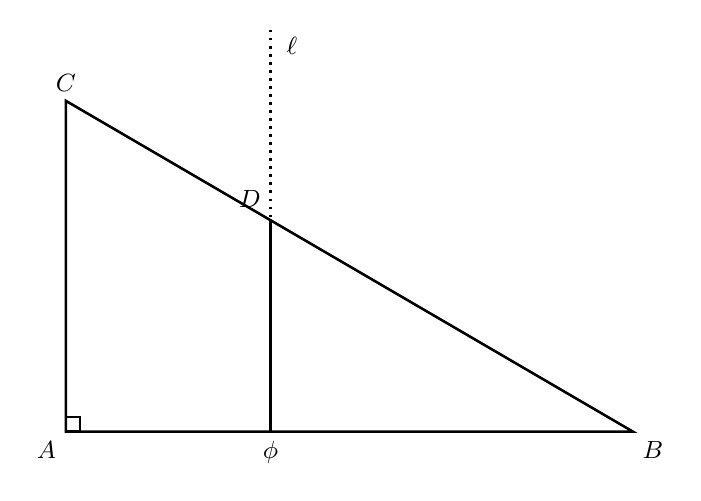
\begin{tikzpicture}[scale=1, font=\small]

      % Internal geometry (not printed)
      \def\b{7.2}        % base length
      \def\H{4.2}        % height
      \def\phival{2.6}   % x-position of dividing line

      % Main triangle vertices
      \coordinate (A)   at (0,0);
      \coordinate (B)   at (\b,0);
      \coordinate (C)   at (0,\H);

      % Intersection of the vertical line with the hypotenuse
      \coordinate (D)   at (\phival, {\H*(1 - \phival/\b)});
      % Intersection with the base
      \coordinate (P)   at (\phival,0);
      % Dotted extension above the triangle
      \coordinate (Top) at (\phival, {\H + 0.9});

      % Triangle
      \draw[line width=0.9pt] (A) -- (B) -- (C) -- cycle;

      % Right-angle mark at A
      \draw[line width=0.8pt]
      (0.18,0) -- ++(0,0.18) -- ++(-0.18,0) -- ++(0,-0.18) -- cycle;

      % Dividing line (solid inside, dotted above)
      \draw[line width=0.9pt] (D) -- (P);
      \draw[dotted, line width=0.9pt] (Top) -- (D)
      node[pos=0.14, right=2pt, yshift=4pt] {\(\ell\)};

      % Sub-segments (consistent weight)
      \draw[line width=0.7pt] (A) -- (P);
      \draw[line width=0.7pt] (P) -- (B);
      \draw[line width=0.7pt] (A) -- (C);
      \draw[line width=0.7pt] (C) -- (D);
      \draw[line width=0.7pt] (D) -- (B);

      % Labels
      \node[below left]          at (A)   {\(A\)};
      \node[below right]         at (B)   {\(B\)};
      \node[above]               at (C)   {\(C\)};
      \node[above left, yshift=1pt] at (D) {\(D\)};
      \node[below]               at (P)   {\(\phi\)};

    \end{tikzpicture}
  \end{center}
  \captionof{figure}{Right-angled triangle \(\triangle ABC\) divided by the line
    \(\ell\).\label{fig:triangle}}

  %--------------------------------------------------------------------------

  \subsection{Problem Four}

  \textbf{\emph{Moscow State University, 1989}}

  In a trapezium \(KLMN\), sides \(KN\) and \(LM\) are parallel, with \(KN=3\) and
  \(\angle M = 120^{\circ}\). \(LM\) and \(MN\) are tangent to the circle
  circumscribed about \(\triangle KLN\). Find the area of \(\triangle KLN\).

  \hfill\textit{[6 Marks]}

  \newpage

  %-----------------------------------------------------------------------------
  \section{Real Analysis}
  %-----------------------------------------------------------------------------

  \subsection{Problem One}

  \textbf{\emph{IMO 2022}}

  Let \(\mathbb{R}^{+}\) denote the set of positive real numbers. Find all
  functions \(f : \mathbb{R}^{+} \to \mathbb{R}^{+}\) such that for each
  \(x \in \mathbb{R}^{+}\), there is exactly one \(y \in \mathbb{R}^{+}\) satisfying
  \[
    x\,f(y) + y\,f(x) \le 2.
  \]

  %=============================================================================
  \chapter{Physics}
  %=============================================================================
  \emph{Definition: Physics,}
  \textbf{The study of all things that exist to place one under mental,
    spiritual, and physical duress.}

  \newpage

  %-----------------------------------------------------------------------------
  \section{Kinematics and Further Mechanics}
  %-----------------------------------------------------------------------------

  \subsection{Problem One}

  \textbf{\emph{Problem Author: Zain Sikand}}

  A person moving at speed \(S\) whistles, stopping once after 5 seconds of
  walking. \(t=15\,\mathrm{s}\) later, he continues walking along his current
  trajectory before passing a stationary group of people. The group of people
  begin to hear the whistling at \(t=30\,\mathrm{s}\) before he passes them.
  Determine the speed at which the man is walking, assuming the
  \textbf{speed of sound \(= 330\,\mathrm{ms}^{-1}\)}.

  \newpage

  %-----------------------------------------------------------------------------
  \section{Astrophysics}
  %-----------------------------------------------------------------------------

  \subsection{Problem One}

  \textbf{\emph{BAAO 2022--23}}
  \newline \\
  The very first image released by the James~Webb Space Telescope (JWST) was of
  a galaxy cluster called SMACS~0723. The image is considered to be Webb's first
  deep field, since a long exposure time of 12.5 hours was used to allow the
  light from very faint and distant galaxies to be seen. The spectrum of one such
  galaxy is shown in Figure~\ref{fig:jwst}.
  \newline \\
  \begin{center}
    \makebox[\textwidth]{%
      \includegraphics[width=1.0\textwidth]{Figure2-1}%
    }
  \end{center}

  \captionof{figure}{Highly redshifted emission lines in the spectrum of a
    galaxy that is 13.1 billion years old, captured using the JWST's
    near-infrared spectrometer (NIRSpec). Credit: NASA, ESA, CSA,
    STScI.\label{fig:jwst}\\}

  The spectrum shows four bright hydrogen lines, which are part of the Balmer
  series (some of which are normally seen in the visible). The rest-frame
  wavelengths of the longest four lines in the series are
  \(410\,\mathrm{nm}\), \(434\,\mathrm{nm}\), \(486\,\mathrm{nm}\), and
  \(656\,\mathrm{nm}\) (\textbf{not all of which are visible in the spectrum}).
  \\
  Once a redshift is known, its recessional velocity can be calculated. At very
  high redshifts, such as these, General Relativity must be used. A conversion
  from redshift to recessional velocity is shown in \ref{fig:conversion}.
  \newline \\
  \begin{enumerate}[label=\alph*)]
    \item Taking measurements from the spectrum, estimate the redshift of the
          galaxy. \emph{(Hint: you should measure more than one line to ensure you
            correctly identify which rest-frame wavelength corresponds to which line.)}

    \item Taking the value of the Hubble constant to be
          \(H_{0} = 70\,\mathrm{km\,s^{-1}\,Mpc^{-1}}\), what is the distance to the
          galaxy? Give your answer in Mpc.
  \end{enumerate}
  \begin{figure}[h]
    \centering
    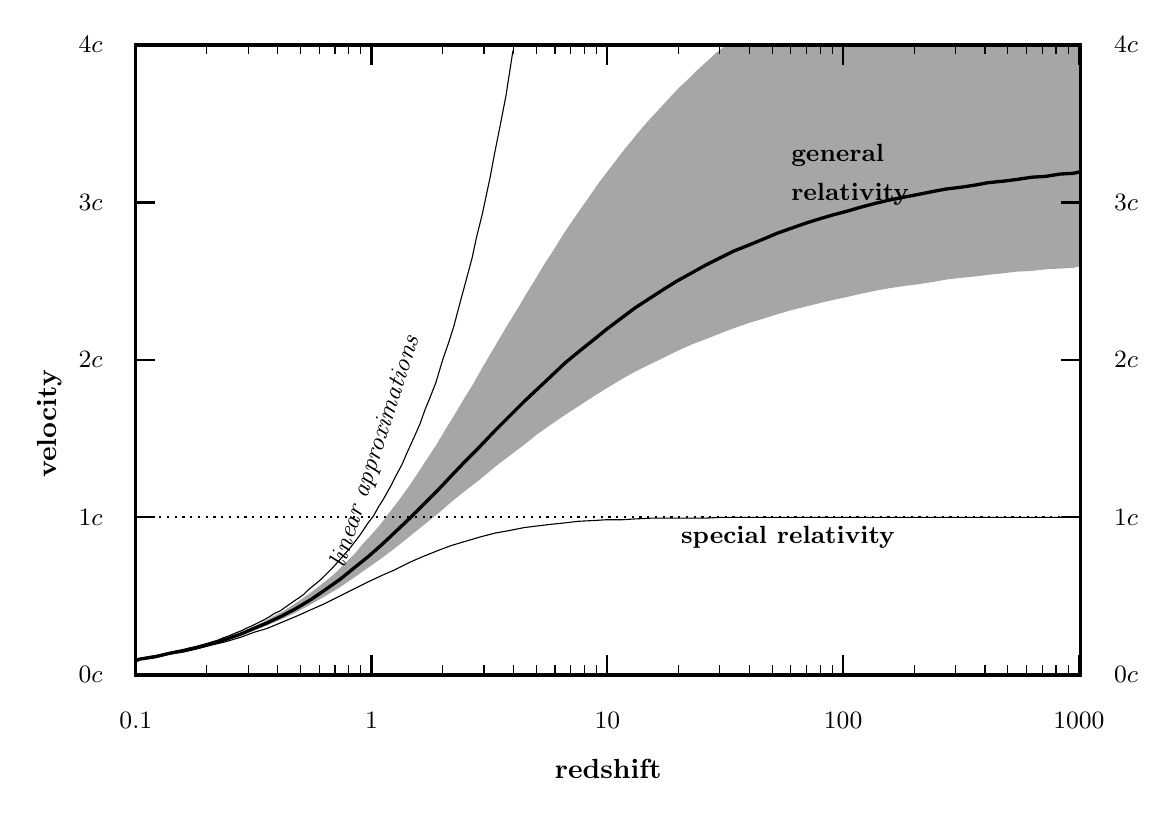
\begin{tikzpicture}[scale=1]
      % Plot-box dimensions (cm)
      %   width  = 12    x ∈ [0, 12]
      %   height =  8    y ∈ [0,  8]
      %
      % Axis mapping (computed externally, baked into coordinates)
      %   x  =  12 · ln(z / 0.1) / ln(10 000)        (log scale)
      %   y  =   8 · (v/c) / 4                        (linear 0–4c)
      %
      % Major-tick x-positions
      %   z = 0.1  →  x = 0       (left edge)
      %   z = 1    →  x = 2.994
      %   z = 10   →  x = 5.988
      %   z = 100  →  x = 8.983
      %   z = 1000 →  x = 11.977  (≈ right edge)

      % --- colour definitions -------------------------------------
      \definecolor{greyband}{gray}{0.65}

      % ============================================================
      %  1.  Grey uncertainty band  (filled region between the two
      %      GR-band-edge curves).  Path = upper edge forward then
      %      lower edge reversed; clipped to the box.
      % ============================================================
      \begin{scope}[clip]
        \clip (0,0) rectangle (12,8);
        \fill[greyband]
        (0.00,0.16) -- (0.00,0.17) -- (0.00,0.19) -- (0.05,0.21) --
        (0.15,0.22) -- (0.28,0.25) -- (0.38,0.27) -- (0.51,0.29) --
        (0.61,0.32) -- (0.74,0.35) -- (0.84,0.38) -- (0.97,0.41) --
        (1.07,0.45) -- (1.21,0.49) -- (1.30,0.53) -- (1.40,0.57) --
        (1.53,0.63) -- (1.63,0.68) -- (1.76,0.75) -- (1.86,0.80) --
        (2.00,0.89) -- (2.09,0.95) -- (2.23,1.05) -- (2.32,1.12) --
        (2.46,1.23) -- (2.56,1.32) -- (2.69,1.45) -- (2.79,1.55) --
        (2.88,1.66) -- (3.02,1.81) -- (3.12,1.93) -- (3.25,2.10) --
        (3.35,2.23) -- (3.48,2.41) -- (3.58,2.56) -- (3.71,2.76) --
        (3.81,2.91) -- (3.94,3.13) -- (4.04,3.29) -- (4.17,3.51) --
        (4.27,3.67) -- (4.40,3.90) -- (4.50,4.07) -- (4.60,4.24) --
        (4.73,4.46) -- (4.83,4.62) -- (4.96,4.84) -- (5.06,5.00) --
        (5.19,5.22) -- (5.29,5.37) -- (5.42,5.58) -- (5.52,5.73) --
        (5.65,5.92) -- (5.75,6.06) -- (5.88,6.25) -- (5.98,6.38) --
        (6.08,6.51) -- (6.21,6.68) -- (6.31,6.80) -- (6.44,6.96) --
        (6.54,7.07) -- (6.67,7.21) -- (6.77,7.32) -- (6.90,7.46) --
        (7.00,7.55) -- (7.13,7.68) -- (7.23,7.77) -- (7.36,7.89) --
        (7.46,7.97) -- (7.59,8.00) --
        % right-edge clip up to top-right corner, across, down
        (12.00,8.00) -- (12.00,5.19) --
        % lower edge (reversed)
        (11.91,5.17) -- (11.74,5.16) -- (11.55,5.15) --
        (11.38,5.13) -- (11.18,5.12) -- (11.02,5.10) --
        (10.82,5.08) -- (10.66,5.06) -- (10.46,5.04) --
        (10.29,5.02) -- (10.13,4.99) -- (9.93,4.96) --
        (9.77,4.94)  -- (9.57,4.91)  -- (9.40,4.88) --
        (9.21,4.84)  -- (9.04,4.80)  -- (8.85,4.76) --
        (8.68,4.72)  -- (8.52,4.68)  -- (8.32,4.63) --
        (8.15,4.58)  -- (7.96,4.52)  -- (7.79,4.47) --
        (7.59,4.40)  -- (7.43,4.34)  -- (7.23,4.26) --
        (7.07,4.20)  -- (6.87,4.11)  -- (6.71,4.03) --
        (6.54,3.95)  -- (6.34,3.85)  -- (6.18,3.76) --
        (5.98,3.64)  -- (5.82,3.54)  -- (5.62,3.41) --
        (5.45,3.30)  -- (5.26,3.17)  -- (5.09,3.05) --
        (4.93,2.92)  -- (4.73,2.77)  -- (4.56,2.64) --
        (4.37,2.48)  -- (4.20,2.35)  -- (4.00,2.19) --
        (3.84,2.05)  -- (3.64,1.89)  -- (3.48,1.76) --
        (3.28,1.60)  -- (3.12,1.48)  -- (2.95,1.36) --
        (2.75,1.22)  -- (2.59,1.11)  -- (2.39,0.99) --
        (2.23,0.90)  -- (2.03,0.79)  -- (1.86,0.71) --
        (1.67,0.63)  -- (1.50,0.56)  -- (1.34,0.50) --
        (1.14,0.44)  -- (0.97,0.39)  -- (0.78,0.34) --
        (0.61,0.30)  -- (0.41,0.26)  -- (0.25,0.23) --
        (0.05,0.20)  -- (0.00,0.18)  -- cycle;
      \end{scope}

      % ============================================================
      %  2.  General-Relativity solid curve  (concordance cosmology)
      % ============================================================
      \draw[very thick, black]
      (0.00,0.16) -- (0.00,0.18) -- (0.05,0.20) -- (0.25,0.23) --
      (0.41,0.27) -- (0.61,0.31) -- (0.78,0.35) -- (0.97,0.40) --
      (1.14,0.45) -- (1.34,0.52) -- (1.50,0.59) -- (1.67,0.66) --
      (1.86,0.75) -- (2.03,0.84) -- (2.23,0.96) -- (2.39,1.07) --
      (2.59,1.21) -- (2.75,1.34) -- (2.95,1.50) -- (3.12,1.65) --
      (3.28,1.80) -- (3.48,1.99) -- (3.64,2.15) -- (3.84,2.35) --
      (4.00,2.52) -- (4.20,2.73) -- (4.37,2.90) -- (4.56,3.10) --
      (4.73,3.27) -- (4.93,3.47) -- (5.09,3.62) -- (5.26,3.78) --
      (5.45,3.96) -- (5.62,4.10) -- (5.82,4.26) -- (5.98,4.39) --
      (6.18,4.54) -- (6.34,4.66) -- (6.54,4.79) -- (6.71,4.90) --
      (6.87,5.00) -- (7.07,5.11) -- (7.23,5.20) -- (7.43,5.30) --
      (7.59,5.38) -- (7.79,5.46) -- (7.96,5.53) -- (8.15,5.61) --
      (8.32,5.67) -- (8.52,5.74) -- (8.68,5.79) -- (8.85,5.84) --
      (9.04,5.89) -- (9.21,5.94) -- (9.40,5.99) -- (9.57,6.03) --
      (9.77,6.07) -- (9.93,6.10) -- (10.13,6.14) -- (10.29,6.17) --
      (10.46,6.19) -- (10.66,6.22) -- (10.82,6.25) -- (11.02,6.27) --
      (11.18,6.29) -- (11.38,6.32) -- (11.55,6.33) -- (11.74,6.36) --
      (11.91,6.37) -- (12.00,6.39);

      % ============================================================
      %  3.  Special-Relativity curve  (thin)
      % ============================================================
      \draw[thin, black]
      (0.05,0.20) -- (0.25,0.23) -- (0.41,0.26) -- (0.61,0.29) --
      (0.78,0.33) -- (0.97,0.38) -- (1.14,0.42) -- (1.34,0.48) --
      (1.50,0.54) -- (1.67,0.59) -- (1.86,0.67) -- (2.03,0.74) --
      (2.23,0.83) -- (2.39,0.90) -- (2.59,1.00) -- (2.75,1.08) --
      (2.95,1.18) -- (3.12,1.26) -- (3.28,1.33) -- (3.48,1.43) --
      (3.64,1.50) -- (3.84,1.58) -- (4.00,1.64) -- (4.20,1.70) --
      (4.37,1.75) -- (4.56,1.80) -- (4.73,1.83) -- (4.93,1.87) --
      (5.09,1.89) -- (5.26,1.91) -- (5.45,1.93) -- (5.62,1.95) --
      (5.82,1.96) -- (5.98,1.97) -- (6.18,1.97) -- (6.34,1.98) --
      (6.54,1.99) -- (6.71,1.99) -- (6.87,1.99) -- (7.07,1.99) --
      (7.23,1.99) -- (7.43,2.00) -- (7.59,2.00) -- (7.79,2.00) --
      (7.96,2.00) -- (8.15,2.00) -- (8.32,2.00) -- (8.52,2.00) --
      (8.68,2.00) -- (8.85,2.00) -- (9.04,2.00) -- (9.21,2.00) --
      (9.40,2.00) -- (9.57,2.00) -- (9.77,2.00) -- (9.93,2.00) --
      (10.13,2.00) -- (10.29,2.00) -- (10.46,2.00) -- (10.66,2.00) --
      (10.82,2.00) -- (11.02,2.00) -- (11.18,2.00) -- (11.38,2.00) --
      (11.55,2.00) -- (11.74,2.00) -- (11.91,2.00) -- (12.00,2.00);

      % ============================================================
      %  4.  Linear-approximation line  v = zc  (thin, clipped)
      % ============================================================
      \draw[thin, black]
      (0.09,0.21) -- (0.15,0.23) -- (0.22,0.24) -- (0.28,0.25) --
      (0.38,0.27) -- (0.45,0.28) -- (0.51,0.30) -- (0.58,0.31) --
      (0.68,0.34) -- (0.74,0.35) -- (0.81,0.37) -- (0.88,0.39) --
      (0.94,0.41) -- (1.04,0.44) -- (1.11,0.47) -- (1.17,0.49) --
      (1.24,0.52) -- (1.34,0.56) -- (1.40,0.59) -- (1.47,0.62) --
      (1.53,0.65) -- (1.63,0.70) -- (1.70,0.74) -- (1.76,0.78) --
      (1.83,0.81) -- (1.90,0.86) -- (2.00,0.93) -- (2.06,0.97) --
      (2.13,1.02) -- (2.19,1.08) -- (2.29,1.16) -- (2.36,1.22) --
      (2.42,1.28) -- (2.49,1.35) -- (2.59,1.46) -- (2.65,1.53) --
      (2.72,1.61) -- (2.79,1.70) -- (2.85,1.78) -- (2.95,1.93) --
      (3.02,2.02) -- (3.08,2.13) -- (3.15,2.24) -- (3.25,2.42) --
      (3.31,2.54) -- (3.38,2.67) -- (3.44,2.81) -- (3.54,3.03) --
      (3.61,3.19) -- (3.67,3.36) -- (3.74,3.53) -- (3.81,3.71) --
      (3.90,4.01) -- (3.97,4.21) -- (4.04,4.43) -- (4.10,4.66) --
      (4.20,5.03) -- (4.27,5.29) -- (4.33,5.57) -- (4.40,5.85) --
      (4.50,6.32) -- (4.56,6.64) -- (4.63,6.99) -- (4.70,7.35) --
      (4.79,7.93);

      % ============================================================
      %  5.  Horizontal dotted line at  v = 1c  (y = 2)
      % ============================================================
      \draw[dotted, thick] (0,2) -- (12,2);

      % ============================================================
      %  6.  Plot-box border  (drawn last so it sits on top)
      % ============================================================
      \draw[very thick, black] (0,0) rectangle (12,8);

      % ============================================================
      %  7.  Tick marks
      %      Left & right y-axis : 0c, 1c, 2c, 3c, 4c  (y = 0,2,4,6,8)
      %      Bottom & top x-axis : 0.1, 1, 10, 100, 1000
      %        mapped to x = 0, 2.994, 5.988, 8.983, 11.977
      % ============================================================

      % --- y-axis ticks (left, inward) ---
      \foreach \yval/\ylabel in {0/0c, 2/1c, 4/2c, 6/3c, 8/4c}
        {
          \draw[thick] (0,\yval) -- (0.25,\yval);
          \node[left, font=\small] at (-0.3,\yval) {\(\ylabel\)};
        }
      % --- y-axis ticks (right, inward) ---
      \foreach \yval/\ylabel in {0/0c, 2/1c, 4/2c, 6/3c, 8/4c}
        {
          \draw[thick] (12,\yval) -- (11.75,\yval);
          \node[right, font=\small] at (12.3,\yval) {\(\ylabel\)};
        }

      % --- x-axis ticks (bottom, inward) ---
      \foreach \xval/\xlabel in {0/0.1, 2.994/1, 5.988/10, 8.983/100, 11.977/1000}
        {
          \draw[thick] (\xval,0) -- (\xval,0.25);
          \node[below, font=\small] at (\xval,-0.35) {\(\xlabel\)};
        }
      % --- x-axis ticks (top, inward) ---
      \foreach \xval in {0, 2.994, 5.988, 8.983, 11.977}
        {
          \draw[thick] (\xval,8) -- (\xval,7.75);
        }

      % --- minor x-ticks (bottom & top) for decades
      %     z = 2..9 inside each decade; positions via ln mapping
      %     decade [0.1,1]  base x=0        scale = 2.994/ln(10) = 1.300
      %     decade [1,10]   base x=2.994    same scale
      %     decade [10,100] base x=5.988
      %     decade [100,1000] base x=8.983
      \foreach \base in {0, 2.994, 5.988, 8.983}
        {
          \foreach \k in {2,3,4,5,6,7,8,9}
            {
              \pgfmathsetmacro{\xm}{\base + 1.300 * ln(\k)}
              \draw[thin] (\xm,0)   -- (\xm,0.12);
              \draw[thin] (\xm,8)   -- (\xm,7.88);
            }
        }

      % ============================================================
      %  8.  Axis labels
      % ============================================================
      \node[left, rotate=90, font=\normalsize] at (-1.1, 4) {\textbf{velocity}};
      \node[below, font=\normalsize]           at (6, -0.95) {\textbf{redshift}};

      % ============================================================
      %  9.  Curve labels  (positioned to match the original figure)
      % ============================================================

      % "linear approximations" — rotated label along the steep line,
      %   placed around x ≈ 3.2, y ≈ 2.5  (mid-rise)
      \node[rotate=72, font=\small, anchor=center]
      at (3.05, 2.85) {\textit{linear approximations}};

      % "special relativity" — right side, just below the dotted 1c line
      \node[font=\small, anchor=west]
      at (6.8, 1.75) {\textbf{special relativity}};

      % "general relativity" — upper right, on the bold curve
      \node[font=\small, anchor=west]
      at (8.2, 6.6) {\textbf{general}};
      \node[font=\small, anchor=west]
      at (8.2, 6.1) {\textbf{relativity}};

    \end{tikzpicture}
    \\
    \caption{%
      Conversion from redshift to recessional velocity for a linear
      approximation (\(v = zc\)), using Special Relativity: \(\left(v = c\,\dfrac{(1+z)^2 - 1}{(1+z)^2 + 1}\right)\)
      ,and using General Relativity:
      \(\left(v = \dot{a}(z)\displaystyle\int_0^z \frac{c\,dz'}{H(z')}\right)\).
      The grey area corresponds to a variety of values for cosmological
      parameters.  The solid line corresponds to values approximately the
      same as the current measured cosmological parameters.
      Credit: Davis \& Lineweaver (2001).
    }
    \label{fig:conversion}
  \end{figure}
  %=============================================================================
  \chapter{Philosophy}
  %=============================================================================

  \newpage

  %-----------------------------------------------------------------------------
  \section{Principles Regarding Infinity}
  %-----------------------------------------------------------------------------

  \subsection{Human Knowledge}

  George Berkeley, in his \emph{Treatise Concerning the Principles of Human
    Knowledge}, explores the idea that man is disillusioned by the
  incomprehensible nature of infinity; a consciousness that is finite is
  incapable of comprehending that of the infinite. From this, he goes on to
  reject the notion of abstract, mind-independent material substance given that
  it is incomprehensible to a finite being. He instead asserts that reality
  consists only of finite minds and infinite minds --- with God's boundless
  perception being the primary reason for the conceptualisation of the infinite.

  Shifting to a mathematical perspective, we see Berkeley reject the
  mathematical interpretations of infinitesimals and infinite quantities; he
  believes them to be incoherent and undefinable within man's finite perception
  of reality. This is seen in how he attacks the notion of \textbf{fluxions},
  referring to them as the \say{\textit{ghosts of departed quantities}}.
  Further exploring this idea of the comprehensibility of that of the infinite,
  we can see that his perspective regarding such critiques the usage of
  abstraction in order to conceptualise. He attacks the notion of
  \say{\textit{infinitely small}} values, enforcing the idea that a
  conceptualisation must stem from real, perceived ideas as opposed to
  abstraction.

  However, Berkeley did not directly oppose the usage of mathematical
  abstraction in reasoning. Despite the fact that he rejected the notion of
  abstraction, he credited the need for a way to quantify infinite concepts and
  acknowledged the practical usage of algebraic methods; but for Berkeley this
  was never the true perception of these principles. His primary focus remained
  on the belief that true knowledge comes from perception, and as such, could not
  philosophically accept the conceptualisation of the imperceivable infinite. As
  such, mathematical concepts that dealt with the infinite were subject to this
  belief until they reduced the infinite to something that is perceivable --- a
  finite quantity.

  \subsubsection{Burning Questions}

  This rejection of abstract conceptualisation regarding the finite thus implies
  that it is impossible for the finite being that is man to idealise infinity;
  however man interacts with infinity in the physical world regularly --- the
  physics explaining our interactions with the world are beyond that of the
  abstract, they are real and applicable. Despite this, they utilise the abstract
  concepts that are imaginary numbers and infinite quantities at the low level. As
  such, how could this philosophical approach reason with physical concepts
  regarding the infinite?

  %--------------------------------------------------------------------------

  \subsection{Mathematical Approaches to the Infinite}

  Aristotle, as one of the early thinkers surrounding infinity, introduced some
  of the foundational abstract concepts that later allowed for mathematical
  practicalisation of infinite quantities. In Book~3 of his works, titled
  \emph{Physics}, he deals with the infinite in regards to actuality and
  potentiality. He states:
  \begin{quote}
    \textit{It is always possible to think of a larger number: for the number of
      times a magnitude can be bisected is infinite. Hence the infinite is
      potential, never actual; the number of parts that can be taken always
      surpasses any assigned number.}
  \end{quote}

  \newpage

  %-----------------------------------------------------------------------------
  \section{Principles Regarding Consciousness in Physics}
  %-----------------------------------------------------------------------------

  \subsection{Quantum Approaches to Consciousness}

  From a physical standpoint, it is widely accepted that the presence of
  consciousness is a result of mental activity within the material brain in some
  way; from this it is legitimate to question the relation this holds with
  quantum theory and, in the process, question whether consciousness is a
  physical property.

  There are several approaches to this, of which we will focus on the following
  primaries:
  \begin{itemize}
    \item Consciousness is a manifestation of quantum processes in the brain.
    \item Quantum concepts are used to understand conscious mental activity
          without referring to brain activity.
    \item Matter and consciousness are regarded as dual aspects of one
          underlying reality.
  \end{itemize}
  \emph{These approaches are further explored in the following from the
    Stanford Encyclopedia of Philosophy~\cite{sep-qt-consciousness}.}

  %--------------------------------------------------------------------------

  \subsection{Traditional Philosophical Concepts}

  In order to explore the quantum aspects of human consciousness and the
  universe's manifestation of itself through consciousness, we must first shift
  to a more traditional perspective so that we may understand the fundamental
  ideas of materialism, the physical existence of the conscious mind, and
  perception of reality.

  Throughout the history of the subject, we see variance in perspectives
  surrounding the dichotomy of mind and matter, from the fundamental
  distinction between primordial descriptions of consciousness, to that of the
  birth of collective consciousness. Kant, as an early thinker regarding human
  perception of reality, states in his \emph{Critique of Practical Reason} that
  both the \say{\textit{starry heavens above and the moral law within me}}.
  Kant, in this conclusion of the critique, essentially draws attention to the
  invisible self and its importance, regarding the importance of man to itself ---
  doing so, he destroys the importance of man in physicality by drawing attention
  to his place in the respective universe. Fundamentally, he attempts to assert
  the idea that when one dies an invisible universe constructed by their own
  consciousness, imagined only by their ideals, dies with them. Resulting from
  this conclusion is Kant's principle surrounding the significance of man's
  existence: human consciousness is inherently irreplaceable and as such the
  conscious perception of the universe for man dies with him.

  \subsubsection{The Materialist Approach}

  The materialist approach to the conceptualisation of consciousness asserts the
  exact counter-argument to Kant's philosophy, reiterating that the
  consciousness of man is irrelevant to his true nature; humans are inherently
  machine-like entities that follow the parameters set out to them by the
  physical world to which they have no influence over. Man blindly follows the
  instructions of the universe, held slave to the world in which he believes
  himself to be in control of, when his idealistic idea of reality is
  fundamentally shaped by his perception of the physical world. However, to say
  that man and machine are one is to reduce the conscious understanding of
  machine: machines grow obsolete, and are lacking in value to humanity should
  their abundance become a nuisance. This approach towards machines does not
  permeate that of the approach towards fellow humans; to say that the conscious
  mind regards its peers as merely machine is a falsehood henceforth. We respect
  the fellow human consciousness regardless of what obsolescence, nuisance, or
  overwhelming abundance it may have. We can divide this materialist approach
  based on how the machine-like nature of man is perceived by a thinker. Popper
  states that they can be divided into two categories:
  \begin{quote}
    \textit{those who deny the existence of mental events, of personal
      experiences, or of consciousness; or who say perhaps that the question
      whether such experiences exist is of minor importance and may be safely left
      open; and those who admit the existence of mental events, but assert that
      they are ``epiphenomena'' --- that everything can be explained without them,
      since the material world is causally closed.}
  \end{quote}

  \subsubsection{Panpsychism}

  The notion of Panpsychism stems from both theoretical Physics and ideas
  brought forth by key thinkers in Philosophy, with its alignment with some
  forms of scientific research marking a key point in perception of the
  conception of consciousness from both perspectives. The panpsychist approach
  brings about the idea that the existence of consciousness is innate within the
  universe, that the very existence of a physical world implies the existence of
  a conscious entity. This can be regarded as the \say{\textit{physicalist
      principle of the closedness of the physical world}}, says Popper --- a set of
  ideas that stem from the physicalist belief that a universe is not open to a
  realm with no conscious perception of itself. Hence, the notion of
  Panpsychism itself implies that the universe observes itself through the
  implied existence of consciousness, with this being the surface-level approach
  to panpsychist thinking. Popper puts this perfectly, stating
  \say{\textit{With the integration of atoms into giant molecules and living
      matter, memory-like effects emerge; and with the higher animals, consciousness
      emerges}}.\footnote{\cite{4d951e62-53cf-3139-b071-86c179b408b8}} He states that
  any form of physicality implies the existence of some form of psychicality.
  Panpsychism believes that consciousness, in its most primitive form, is an
  innate quality and as such, mind implies matter and vice versa.
  <<<<<<< Updated upstream

  =======
  \newline \\
  >>>>>>> Stashed changes
  This philosophy permeates even that of the inanimate, with the belief being
  that they lie in states described as \say{\textit{pre-psychical}} or
  \say{\textit{proto-psychical}}. This philosophy regarding consciousness
  predates modern metaphysics and quantum theory. Despite its age, it asserts a
  quantum approach to consciousness: observation is needed for the existence of a
  deterministic physical outcome in our universe at the quantum level. A universe
  lacking conscious observation is one that is purely theoretical, one that
  cannot be physically certain for every possible aspect of its existence can be
  reduced to something purely probabilistic, as per quantum uncertainty.
  Heisenberg ascribes to the notion of quantum uncertainty the notion of
  fundamental indeterminacy: the wave-particle duality of matter and
  probabilistic outcome of atomic properties leads him to believe this. This, of
  course, makes perfect sense --- the man who created the quantum uncertainty
  principle will of course reject universal determinism. However, I believe that,
  ultimately, the notion of Panpsychism provides a means to an ultimately
  deterministic outcome in the universe despite its probabilistic nature.

  \printbibliography

\end{raggedright}
\end{document}